%!TEX root = ../thesis.tex
%*******************************************************************************
%****************************** Second Chapter *********************************
%*******************************************************************************

\chapter{Περιδινούμενες ροές σε αγωγούς}\label{ch:swirlflows}

\begin{chapquote}{H. Melville, \textit{Moby Dick}}
“The bed was soft enought to suit me\dots But I soon found that there came such a draught of cold air over me from the sill of the window that this plan would never do at all, especially as another current from the rickety door met the one from the window and both together formed a series of small whirlwinds in the immediate vicinity of the spot where I had thought to spend the night.”
\end{chapquote}

\ifpdf
    \graphicspath{{Chapter2/Figs/Vector/}{Chapter2/Figs/PDF/}{Chapter2/Figs/}}
\else
    \graphicspath{{Chapter2/Figs/Raster/}{Chapter2/Figs/}}
\fi


% ******************************* Nomenclature ****************************************
\nomenclature[a-S]{S}{Αριθμός στροβιλισμού}

\noindent Ως ροή στροβιλισμού ορίζεται οποιαδήποτε ροή που έχει περιστροφική κίνηση. Μερικά παραδείγματα ροών που εμπίπτουν σε αυτή την κατηγορία είναι οι διαχωριστές κυκλώνων, οι φυσικοί ανεμοστρόβιλοι, ορισμένοι εναλλάκτες θερμότητας και κινητήρες καύσης \cite{1984_Gupta_BOOK}.

Οι στροβιλώδεις (ή περιδινούμενες) ροές αποτελούν αντικείμενο εντατικών ερευνών τα τελευταία χρόνια. Το κύριο χαρακτηριστικό τους έγκειται στη σημαντική βελτίωση μεταφοράς θερμότητας και μάζας που μπορούν να πετύχουν, ελαχιστοποιώντας παράλληλα το ενεργειακό κόστος.

Χρησιμοποιούνται σε ένα ευρύ εφαρμογών, όπως εναλλάκτες θερμότητας και μάζας \parencites{1976_Hong}{1986_Walsh}{2002_Bsebsu}, τουρμπίνες καύσης \cite{1986_Lede}, πυραύλους ή διαχωριστές που χρησιμοποιούν φυγοκεντρικά φαινόμενα, όπως οι κυκλώνες και οι υδροκυκλώνες, προκειμένου να απομακρύνουν σωματίδια ή σταγονίδια από μείγματα \cite{1986_Akiyama}. Είναι επίσης μια δημοφιλής μέθοδος σταθεροποίησης της φλόγας σε πολλά βιομηχανικά συστήματα καύσης \cite{2020_Δόγκας_DISSERTATION}, αλλά και της αποτελεσματικής αντιμετώπισης του προβλήματος της υπερθέρμανσης (στη περιοχής σύνδεσης πτερυγίου – δαπέδου) σε αεριοστρόβιλο \cite{2015_Μηλιδόνης_DISSERTATION}.

Πρόσφατα έχουνε εφαρμοστεί και σε συστήματα πνευματικής μεταφοράς προκειμένου να μειώσουν τη πίεση που προκαλείται από καθίζηση σωματιδίων, και να αποφευχθεί πιθανή φραγή \parencites{1996_Li}{1994_Li}. Έχει επίσης μελετηθεί η χρήση στροβίλου για την εναπόθεση μικρών πετρωμάτων από γεωτρύπανο κατά τη διάρκεια της γεώτρησης \cite{2019_Qu}. Η δημιουργία ενός τύπου περιδινούμενης ροής σε έναν θάλαμο καύσης δύναται να βελτιώσει την ποιότητά της \cite{1996_Sheen}.

Από τις πρώτες μελέτες που πραγματεύτηκαν τις περιδινούμενες ροές ήταν αυτή του \citeauthor{1954_Talbot} \cite{1954_Talbot}, ο οποίος παρατήρησε ότι η περιστροφική κίνηση ενός υγρού που προκαλείται από τη περιστροφή του τμήματος εισόδου του εσωτερικού κυλίνδρου ενός δακτυλιοειδούς σωλήνα, δημιουργεί εφαπτομενική ροή η οποία φθίνει κατά μήκος του σωλήνα, δημιουργώντας αστάθειες που μπορούν να ερμηνευθούν ως κατακρήμνιση δινών\footnote{ο αγγλικός όρος είναι: ruptures of swirling eddies} \cite{1991_Bottaro}. Παρατηρήθηκε ότι η ροή αυτή ήταν αρκετά σύνθετη, παρουσιάζοντας έντονη τριδιάστατη συμπεριφορά και χαρακτηριζόταν από καμπύλες γραμμές ροής, συνεπώς διέφερε σημαντικά από αξονικές ροές - ειδικά στην περιοχή πλησίον των τοιχωμάτων \cite{1988_Yowakim}.

\section{Γενέτειρες στροβιλισμού}

\noindent Μεγάλος αριθμός μελετών έχει πραγματευτεί τη δημιουργία περιδινούμενης ροής, χρησιμοποιώντας ποικίλες μεθόδους όπως: (i) με εισαγωγή του ρευστού μέσω μίας (ή περισσότερων) εφαπτομενικής(-ών) εισόδου(-ών), (ii) με πτερύγια οδηγούς που παρεμβάλλονται ακτινικά μεταξύ δύο δίσκων στο τμήμα εισόδου ενός σωλήνα, (iii) με περιστροφή ενός τμήματος ενός σωλήνα ή μίας διακτυλιοειδούς διάταξης και (iv) με την απότομη διαστολή ενός σωλήνα αξονικής ροής, όπως για παράδειγμα σε θάλαμο καύσης \cite{1995_Hallett}.

Όσον αφορά τη μέθοδο εφαπτομενικών εισόδων (\prettyref{fig:tangin}), έχει χρησιμοποιηθεί σε αρκετές έρευνες πειραματικής φύσεως \parencites{1961_Nissan}{1985_Shoukry}{2003_McClusky_CONF}{1990_Legentilhomme}{1991_Legentilhomme}{1993_Kumar}, στις οποίες ο αριθμός εισόδων που χρησιμοποιείται κυμαίνεται από μία \cite{1975_Hay} έως 224 \cite{1984_Sparrow}. Η μια εφαπτομενική είσοδος παρήγαγε ασύμμετρη ροή, ενώ η ύπαρξη μόνο δύο εισόδων στις 180 μοίρες παρήγαγε συμμετρικό στροβιλισμό \parencites{1961_Nissan}{1980_Ito}. Επίσης, σύμφωνα με τους \citeauthor{1991_Legentilhomme} \cite{1991_Legentilhomme}, η προκαλούμενη περιδίνηση διαφέρει αισθητά ανάλογα με το λόγο πάχους του δακτυλίου, $\left(R_{\text{εξ.}} - R_{\text{εσ.}}\right)$, προς τη διάμετρο των βρόγχων, $\left(D_{\beta}\right)$, και διακρίνεται σε τρία είδη: (i) κανονική περιδινούμενη ροή (pure swirl flow) όταν $R_{\text{εξ.}} - R_{\text{εσ.}} = D_{\beta}$, (ii) συστολική περιδινούμενη ροή (contraction swirl flow) όταν $R_{\text{εξ.}} - R_{\text{εσ.}} < D_{\beta}$  και (iii) διασταλτική περιδινούμενη ροή (expansion swirl flow) όταν $R_{\text{εξ.}} - R_{\text{εσ.}} > D_{\beta}$.
	
\begin{figure}[htbp]
\centering
\subcaptionbox{Τομή βάσης εφαπτομενικών εισόδων \cite{1995_Chang}}	
  [.4\linewidth]{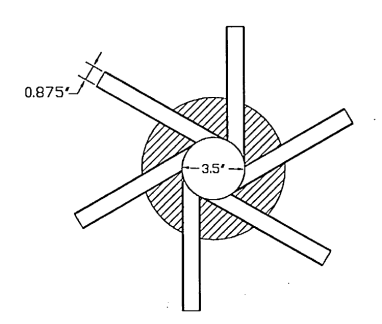
\includegraphics[width=0.4\textwidth]{tangentialinlet1.png}}
\subcaptionbox{Βάση διασταλτικής περιδίνησης \cite{1991_Legentilhomme}}
  [.5\linewidth]{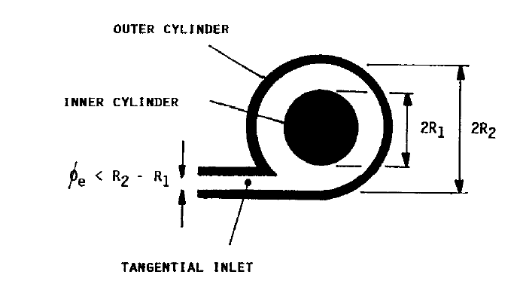
\includegraphics[width=0.5\textwidth]{tangentialinlet2.png}}
\caption{Περιδίνηση με χρήση βάσεων εφαπτομενικών εισόδων}\label{fig:tangin}
\end{figure}

Πολλά ερευνητικά έργα \parencites{1976_Murakami}{1975_Zaherzadeh}{1986_Morsi} έχουν χρησιμοποιήσει οδηγούς-πτερύγια. Αυτά ισαπέχουν γύρο από την είσοδο της εγκατάστασης και προσδίδουν εφαπτομενική ταχύτητα στη ροή (\prettyref{fig:gvanes}). Η ισχύς της συνιστώσας στροβιλισμού μπορεί να μεταβληθεί ρυθμίζοντας τη γωνία των πτερυγίων και η ομοιομορφία του πεδίου ροής μπορεί επίσης να βελτιωθεί με την αύξηση του αριθμού των πτερυγίων.

\begin{figure}[htbp]
\centering
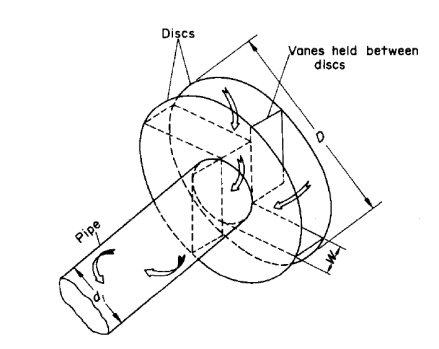
\includegraphics[scale=1]{guidedvanes.png}
\caption{Βάση περιδίνησης χρησιμοποιώντας οδηγούς-πτερύγια \cite{1975_Zaherzadeh}}\label{fig:gvanes}
\end{figure}

Η τεχνική των περιστρεφόμενων τμημάτων \parencites{1976_Murakami}{1954_Talbot}{1976_Crane}, η οποία προκαλεί στροβιλισμό με αντίσταση τριβής από ένα περιστρεφόμενο τοίχωμα, δημιουργεί ασθενή στροβιλισμό εάν χρησιμοποιηθεί σε απλή κυλινδρική διατομή. Οι \citeauthor{1976_Murakami} \cite{1976_Murakami} χρησιμοποίησαν μια ακτινική πτερωτή η οποία περιστρεφόταν μαζί με τον σωλήνα και δημιουργούσε μια ισχυρή δίνη κατά μήκος της ροής. Στις δακτυλιοειδείς ροές, η δημιουργία στροβιλισμού από την περιστροφή των εσωτερικού και του εξωτερικού κυλίνδρων έχει μελετηθεί εκτενώς από τον \citeauthor{1935_Taylor} \cite{1935_Taylor} ο οποίος χρησιμοποίησε ένα σύστημα ομόκεντρων κυλίνδρων, με τον εσωτερικό να περιστρέφεται, για να διερευνήσει το πώς εξελίσσεται ο στροβιλισμός κατά μήκος του αγωγού.

Τούτων λεχθέντων, η μακράν πιο συνηθισμένη διάταξη παραγωγή στροβιλισμού είναι μέσω συστραμμένης ταινίας (twisted tape) (\prettyref{fig:twisttape}) \parencites{1976_Hong}{2021_Wang}{2001_Manglik}. Ταινίες, πλάτους ίσου με τη διάμετρο του σωλήνα, συστρέφονται γύρο από το διαμήκη άξονα και εισάγονται σε σωλήνα, αναγκάζοντας το εργαζόμενο μέσο να περιστρέφεται μαζί με την ταινία. Το πεδίο ροής που παράγεται από την ταινία είναι πολύ διαφορετικό από εκείνο των εφαπτομενικών μεθόδων στροβιλισμού. Για αρχή, η συστραμμένη ταινία διαιρεί τη ροή σε δύο μικρότερες ημικυκλικής διατομής, οπότε δεν μπορεί να χαρακτηριστεί ως αξονοσυμμετρική. Η αυξημένη βρεγμένη επιφάνεια προκαλεί ανάπτυξη οριακών στρωμάτων που διαταράσσουν το πεδίο ροής και αυξάνουν αισθητά τον συντελεστή τριβής. Έχουν παρατηρηθεί επίσης σημαντικές διακυμάνσεις στα χαρακτηριστικά μεταφοράς θερμότητας της ροής.

\begin{figure}[htbp]
\centering
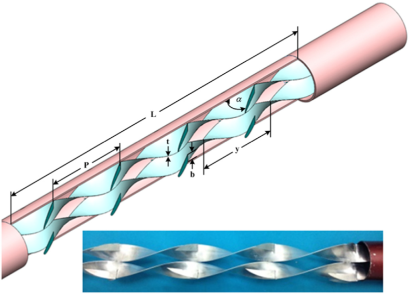
\includegraphics[scale=1]{twistedtape.png}
\caption{Δύο συστραμμένες ταινίες στην πειραματική διάταξη των \citeauthor{2016_Tamna} \cite{2016_Tamna}}\label{fig:twisttape}
\end{figure}

\section{Ποσοτικοποίηση στροβιλισμού}

\noindent Βασικό χαρακτηριστικό των περιδινούμενων ροών, που δημιουργούνται μέσω κάποιας διάταξης τοποθετημένης στην αρχή της ροής, είναι η εξασθένιση του στροβιλισμού κατά μήκος της διαδρομής της ροής λόγω της μείωσης της γωνιακής συνιστώσας της ταχύτητας. Ο συνήθης τρόπος ποσοτικοποίησης της στροβιλότητας είναι ο αριθμός στροβιλισμού (swirl number) \parencites{1984_Gupta_BOOK}{1998_FariasNeto}. Συμβολίζεται με το γράμμα S και είναι ο λόγος της εφαποτμενικής προς την αξονική ορμή:

\begin{equation}\label{eq:swirl}
S = \displaystyle\frac{\displaystyle\int_{0}^{R} u_z u_{\theta} r^2 \, dr}{R\displaystyle\int_{0}^{R} \left( u_z^2 - \frac{1}{2} u_{\theta}^2 \right)r \, dr}
\end{equation}

\noindent όπου $R$ η ακτίνα του αγωγού και $u_z,\, u_{\theta}$ η αξονική και η εφαπτομενική ταχύτητα για την ακτινική διεύθυνση αντίστοιχα.

\section{Θερμαινόμενες στροβιλώδεις ροές}

\noindent Οι πρώτες πειραματικές μελέτες που αξιοποίησαν διατάξεις δημιουργίας στροβιλισμό ο οποίος εξασθενεί κατά μήκος της ροής σωλήνα δακτυλιοειδούς διατομής είναι έξι στο σύνολό τους, όπως αναφέρει ο \citeauthor{1992_Solnordal_DISSERTATION} \cite{1992_Solnordal_DISSERTATION}. Όλες αυτές οι έρευνες προσδιόριζαν, μεταξύ άλλων, τον συντελεστή μετάδοσης θερμότητας των τοιχωμάτων του συστήματος κοιλοτήτων.

O τοπικός συντελεστής μεταφοράς θερμότητας, όπως αυτές έδειξαν, είναι συνυφασμένος με την απόσταση από τη γενέτειρα ροής $\left(x/d\right)$, τον αριθμό Reynolds $\left(Re\right)$, την ένταση στροβιλισμού $\left(S\right)$ και το πηλίκο θερμοκρασίας ρευστού προς την θερμοκρασία θερμαινόμενης επιφάνειας $\left(T_{\text{αντ}}/T_{\text{ρευ}}\right)$. Όλες αυτές οι μελέτες υπολόγισαν τον τοπικό αριθμό Nusselt και εν συνεχεία άλλαζαν τις προαναφερθείσες παραμέτρους προσπαθώντας να εξάγουν μια συσχέτιση. Μια κοινή παρατήρηση ήταν ότι ο τοπικός συντελεστής συναγωγής αυξανόταν με αντίστοιχη αύξηση των αριθμού Reynolds και της έντασης στροβιλισμού \parencites{1970_Blackwelder}{1973_KlepperO._CONF}{1975_Hay}{1984_Prata}, ενώ οι \citeauthor{1973_KlepperO._CONF} \cite{1973_KlepperO._CONF} και \citeauthor{1970_Blackwelder} \cite{1970_Blackwelder} παρατήρησαν ότι ο αριθμός Nusselt αυξανόταν όσο μεγαλύτερη ήταν η θερμοκρασιακή διαφορά μεταξύ ρευστού και κοιλότητας.

\subsection{Βελτίωση μετάδοσης θερμότητας}

\noindent Σε όλες τις έρευνες βρέθηκε ότι ο τοπικός συντελεστής μεταφορά θερμότητας μειωνόταν εκθετικά \parencites{1970_Blackwelder}{1973_KlepperO._CONF}{1975_Hay}{1984_Prata}, πράγμα που σημαίνει ότι η ενίσχυση μετάδοσης θερμότητας ήταν άμεσα συνυφασμένη με τη γωνιακή συνιστώσα της διατμητικής τάση του τοιχώματος, και ως εκ τούτου, με τον αριθμό στροβιλισμού.

Ο \citeauthor{1970_Blackwelder} \cite{1970_Blackwelder} βρήκε ότι η ενίσχυση μετάδοσης θερμότητας άρχισε να μειώνεται σημαντικά σε μήκος 60 με 80 διαμέτρους κατάντη της γενέτειρας ροής της πειραματικής του διάταξης, για αριθμούς Reynolds μέχρι \num{90e+3}. Οι \citeauthor{1975_Hay} \cite{1975_Hay}, χρησιμοποιώντας μικρότερους αριθμούς Reynolds και περισσότερη ένταση στροβιλισμού, βρήκαν ότι η ενίσχυση μετάδοσης θερμότητας μειώθηκε γύρω στο \qty{25}{\percent} της αρχικής της τιμής, σε μήκος 17.5 διαμέτρων κατάντη της ροής. 

Οι \citeauthor{1975_Zaherzadeh} \cite{1975_Zaherzadeh} έδειξαν ότι η ενίσχυση μετάδοσης θερμότητας μπορούσε να φτάσει μέχρι και το \qty{80}{\percent}. Οι \citeauthor{1975_Hay} \cite{1975_Hay} και οι \citeauthor{1984_Prata} \cite{1984_Prata} υπολόγισαν ενίσχυση μετάδοσης θερμότητας της τάξεως του \qty{500}{\percent} στην έξοδο των γενετειρών στροβιλισμού τους. Αμφότερες μελέτες χρησιμοποίησαν ιδιαίτερα υψηλές τιμές στροβιλισμού.

Η εμπειρική σχέση των \citeauthor{1975_Hay} \cite{1975_Hay} ήταν συναρτήσει του αριθμού στροβιλισμού, S (\prettyref{eq:hay}). Αυτή η συσχέτιση περιγράφει τα δεδομένα τους με ακρίβεια \qty{\pm 40}{\percent}. Αν και η αβεβαιότητα ήταν εκτός αποδεκτών ορίων (όπως καλή ώρα και τα δικά μας αποτελέσματα αργότερα), είναι λογικό δεδομένης της απλοϊκότητας του μοντέλου:
 
\begin{equation}\label{eq:hay}
\displaystyle\frac{Nu}{Nu_{ax}} = \left(S + 1\right)^{1.75}
\end{equation}

\noindent Οι \citeauthor{1970_Blackwelder} \cite{1970_Blackwelder} και \citeauthor{1973_KlepperO._CONF} \cite{1973_KlepperO._CONF} βρήκαν ότι οι τοπικοί συντελεστές συναγωγής ήταν συνυφασμένοι με την θερμοκρασιακή διαφορά ρευστού και τοιχώματος. Αμφότεροι χρησιμοποίησαν ιδιαίτερα υψηλές τιμές ροής θερμότητας, εντείνοντας την θερμοκρασιακή διαφορά. O διάταξη του \citeauthor{1970_Blackwelder} είχε $T_{\text{αντ}}/Τ_{\text{ρευ}} \le 2.1$ ενώ αυτή του \citeauthor{1973_KlepperO._CONF}, $T_{\text{αντ}}/Τ_{\text{ρευ}} = 1.5$.

Επιπλέον, ο \citeauthor{1970_Blackwelder} \cite{1970_Blackwelder} εφήρμοσε γραμμική παλινδρόμηση στα δεδομένα του, για συγκεκριμένο αριθμό Reynolds, χρησιμοποιώντας:

\begin{equation}\label{black}
\displaystyle\frac{Nu}{Nu_{ax}}\left(\displaystyle\frac{T_{\text{αντ}}}{T_{\text{ρευ}}} \right)^{A\frac{x}{d}} \quad \text{με} \quad \displaystyle\frac{x}{d}
\end{equation}

\noindent όπου Α σταθερά που εξαρτάται από την κλίση της συστραμμένης ταινίας. Για αξονικές ροές, ο \citeauthor{1973_KlepperO._CONF} \cite{1973_KlepperO._CONF} συσχέτισε, για πλήρως αναπτυγμένη ροή, τον αριθμό Nusselt με μια τροποποιημένη εξίσωση των \citeauthor{1930_Dittus} \cite{1930_Dittus}:

\begin{equation}\label{eq:dittus}
Nu_{ax} = 0.023 Re^{0.8} Pr^{0.4} \left(\displaystyle\frac{T_{\text{αντ}}}{T_{\text{ρευ}}}\right) ^ {-0.5}
\end{equation}

\noindent Τροποποιώντας την έκφραση αυτή, εξήγαγαν συσχέτιση για τους τοπικούς Nusselt σε περιδινούμενη ροή που φθίνει:

\begin{align}\label{eq:klepp}
Nu_{ax} &= 0.023 Re^{0.8} Pr^{0.4} \left(\displaystyle\frac{T_{\text{αντ}}}{T_{\text{ρευ}}}\right) ^ {-0.5} a b\\[2pt]
a &= \displaystyle\frac{0.7 + 4.2x \num{e-5}Re}{1 + 3.9x \num{e-5}Re}\nonumber\\[2pt]
b &= 1 + \displaystyle\frac{1.05}{\left\{0.5\frac{p}{d_o} + 1.25x\num{e-3}\frac{p}{d_o}\left( \frac{x}{d_o} \right)^2 \right\}^{0.6}}\nonumber
\end{align}

\noindent όπου ο όρος $a$ ισχύει για εύρη Reynolds \num{20e+3} με \num{380e+3} και ο όρος $p$ είναι η περίμετρος της συστραμμένης ταινίας. Τα δεδομένα του \citeauthor{1973_KlepperO._CONF} προσεγγίζονται από την ανωτέρω συσχέτιση με ακρίβεια \qty{\pm 10}{\percent}.

Να σημειωθεί εδώ ότι τα πειραματικά δεδομένα του \citeauthor{1973_KlepperO._CONF} ήταν πάρα πολλά, εκατοντάδες, και κάλυπταν ένα ευρύ φάσμα παραμέτρων (Re από \num{20e+3} μεχρι \num{380e+3}, $p/d_o$ από 4.76 μέχρι 8.05, $T_{\text{αντ}}/T_{\text{ρευ}}$ από 1 μέχρι 2.1). Τα δεδομένα του \citeauthor{1973_KlepperO._CONF} φαίνεται να συμφωνούν με αυτά άλλων δημοσιεύσεων, οπότε η εξίσωση αυτή είναι μια καλή προσέγγιση για περιδινούμενες ροές με χρήση συστραμμένων ταινιών.

Η προσέγγιση των \citeauthor{1971_Narezhnyy} \cite{1971_Narezhnyy} ήταν λίγο διαφορετική. Επειδή τα οριακά στρώματα εξελίσσονται κατά μήκος του σωλήνα, έκριναν πως η συσχέτιση μεταξύ των αριθμών Nusselt και Reynolds θα εξαρτιόταν από την εκάστοτε απόσταση των γενετειρών στροβιλισμού.

Παρατηρώντας τους τοπικούς Nusselt, $Nu_x$, να μεταβάλλονται αναλογικά με ${Re}_x^{0.8}$ όπως στην εξίσωση Dittus-Boelter \cite{1930_Dittus}, προσπάθησαν να βρούνε μια συσχέτιση της μορφής:

\begin{equation}\label{eq:dittuss}
Nu_x = c Re_x^{0.8}
\end{equation}

\noindent όπου η σταθερά c θεωρήθηκε ότι εξαρτιόταν της απόσταση, κατά μήκος της διάταξης, από την γενέτειρα στροβιλισμού και γωνίας εισροής ρευστού. Προσπαθώντας να προσαρμόσουν λοιπόν τα δεδομένα σε αυτού του είδους την εξίσωση κατέληξαν:

\begin{equation}
Nu_x = c_{ax} \left( 1 + tan \phi \right) ^ {0.8 exp\left( -0.0027\frac{x}{d_o} \right)} Re_x^{0.8}
\end{equation}

\noindent η ανωτέρω εξίσωση είναι εφαρμόσιμη για εύρη τοπικών Reynolds από \num{8e+4} με \num{e+7}, $\phi \le \ang{75}$, και $x/d_o \le 150$, ενώ η ακρίβεια της κυμαίνεται στο \qty{\pm 25}{\percent}.

\subsection{Πεδίο ροής}

\noindent Ένα σημαντικό χαρακτηριστικό των διατάξεων με στροβιλισμό έγκειται, όπως και αναφέρθηκε πιο πάνω, στο πολύπλοκο πεδίο ροής που δημιουργείται λόγω μίας κεντρικής ζώνης ανακυκλοφορίας \cite{2003_AlAbdeli}.

\noindent Μία από τις πρώτες προσπάθειες διερεύνησης του πεδίου ροής περιδινούμενων ροών που φθίνουν έγινε από τους \citeauthor{1961_Nissan} \cite{1961_Nissan}. Αυτοί μελέτησαν πειραματικά σωλήνα δακτυλιοειδούς διατομής όπου η περιδίνηση δημιουργείτο από δύο, αντίθετα τοποθετημένες, εφαπτομενικές εισόδους. Παρατήρησαν ότι το πεδίο ταχύτητας χωριζόταν σε τρεις διαφορετικές ζώνες ανάλογα τη μορφολογία του: (i) κοντά στον άξονα, η γωνιακή συνιστώσα της ταχύτητας αυξανόταν με την απομάκρυνση από τον άξονα, ενώ η αξονική γινόταν αρνητική, το οποίο υποδηλώνει την ύπαρξη αντιστρεπτής ροής, (ii) με την απομάκρυνση από τον άξονα υπήρξε αύξηση της γωνιακής ταχύτητας ενώ μηδενιζόταν η αξονική - εδώ, κοντά στον άξονα, υπάρχει πάλι αντιστροφή ροής και τέλος (iii) κοντά στο τοίχωμα, η γωνιακή ταχύτητα μειωνόταν απότομα ενώ η αξονική αυξανόταν. Η αποτύπωση των ζωνών ταχύτητας φαίνεται στο \prettyref{fig:nissan}.

\begin{figure}[htbp]
\centering
\subimport{Chapter2/Figs/pdftex}{nissan.pdf_tex}
\caption[Ζώνες πεδίου ταχύτητας περιδινούμενων ροών]{Οι τρεις διαφορετικές ζώνες ταχυτήτων που δημιουργούνται από στροβιλισμό σε σωλήνα \cite{1961_Nissan}. Οι συνεχείς γραμμές απεικονίζουν την κατανομή πίεσης στην αξονική απόσταση z, ενώ οι διακεκομμένες την κατανομή πίεσης στην απειροστή μεταβολή z + dz.}\label{fig:nissan}
\end{figure}

Επιπλέον, σε μια δακτυλιοειδή περιδινούμενη ροή που προκαλείται με τη βοήθεια οδηγών πτερυγίων, οι \citeauthor{1986_Morsi} \cite{1986_Morsi} έδειξαν ότι το εφαπτομενικό προφίλ ταχύτητας μοιάζει με αυτό εξαναγκασμένης δίνης η οποία τείνει προς το εσωτερικό τοίχωμα και φαίνεται να μειώνεται γραμμικά ενώ πλησιάζει τον εξωτερικό κύλινδρο. Αναλυτικότερα: η αξονική συνιστώσα της ταχύτητας φαινόταν να ακολουθεί ροή περιδίνησης, αλλά μεταβαλλόταν ριζικά κατά μήκος της διαδρομής της. Υψηλότερες αξονικές ταχύτητες εντοπίστηκαν κοντά στον εσωτερικό κύλινδρο, και αυτές φαίνονταν να μειώνονται με τη αύξηση της αξονικής απόστασης από το τμήμα εισόδου του δακτυλίου. Αυτά τα δεδομένα επιβεβαιώθηκαν πειραματικά και από τους \citeauthor{1991_Bottaro} \cite{1991_Bottaro} για ίδια διάταξη και συνθήκες στρωτής ροής, όπου η έγχυση ρευστού γινόταν μέσω μίας εφαπτομενικής εισόδου, καθώς επίσης και από τους \citeauthor{1990_Khodadadi} \cite{1990_Khodadadi}, οι οποίοι έκαναν ακριβώς τις ίδιες παρατηρήσεις, για παρόμοια διάταξη, σε συνθήκες τυρβώδους ροής.

\section{Στόχος παρούσας εργασίας}

\noindent Στην παρούσα εργασία, για την πειραματική διερεύνηση της βελτίωσης μετάδοσης θερμότητας, χρησιμοποιήθηκε στροβιλισμός σε σωλήνα δακτυλιοειδούς διατομής, ο οποίος εξασθενεί όσο εξελίσσεται η ροή. Η εν λόγω ροή δημιουργείτο από ειδικά διαμορφωμένες βάσεις που φέρουν εφαπτομενικές εισόδους ροής και είναι τοποθετημένες ανάντη της διάταξης -  παρόμοια με αυτή των \citeauthor{1995_Chang} \cite{1995_Chang}. Επίσης, ο λόγος πάχους του δακτυλίου που σχηματίζουν οι ομόκεντροι κύλινδροι, $\left(R_{\text{εξ.}} - R_{\text{εσ.}}\right)$, ισούται με τη διάμετρο των βρόγχων, $\left(D_{\beta}\right)$, ώστε να εξασφαλίζονται συνθήκες ροής "pure swirl flow" \cite{1991_Legentilhomme}.

Αυτού του είδος η διάταξη ήταν σχετικά εύκολο να σχεδιαστεί και να συντηρηθεί διότι δεν περιλάμβανε κινητά μέρη - όπως περιστρεφόμενους κυλίνδρους - και προκαλεί εν γένει ασθενέστερη πτώση πίεσης σε σύγκριση με τη μέθοδο οδηγών πτερυγίων. Επιπλέον η χρήση της εφαπτομενικής εισόδου καθιστά εύκολη την στεγανοποίηση της διάταξης. Το κύριο μειονέκτημα αυτών των ροών, ωστόσο, είναι ότι η ροή εξελίσσεται κατά μήκος της διαδρομής με φθίνοντα ρυθμό, όπου και παρατηρείται μείωση των συντελεστών μεταφοράς \parencites{1990_Legentilhomme}{1991_Legentilhomme}{1985_Shoukry}.

Για την ποσοτικοποίηση της βελτίωσης μετάδοσης θερμότητας, αναγκαία ήταν η χρήση συσχέτισης $\overline{Nu} = f(Re)$ για τον προσδιορισμό των αντιπροσωπευτικών Nusselt (βλ. υποενότητα \ref{repnu}). Για τον σκοπό αυτό χρησιμοποιήθηκε η πιο απλή από τις προαναφερθείσες συσχετίσεις, μια παρόμοια αυτής των Dittus-Boelter \cite{1930_Dittus}. Η αποτίμηση της επιλογής αυτής θα γίνει με το πέρας των υπολογισμών, όπου θα έχει προηγηθεί στατιστική ανάλυση, και θα φανεί η αβεβαιότητα στα τελικά αποτελέσματα.